% \chapter{电网脆弱性研究的关键问题与模型验证分析}
\chapter{基于复杂网络的电网模型关键问题研究}
\label{cha:model}

\section{引言}
\label{sec:index2}
% 经典的电力系统分析是基于基尔霍夫电流电压方程、固定的拓扑结构来进行分析的。其研究已形成了较为完善的体系\cite{refs60}。随着科学技术的不断发展,电力系统
% 变得越来越复杂、规模越来越大。在网络拓扑和分析计算上,经典的电力网络分析方法因节点和线路复杂度高的问题已不再适用。
从复杂网络角度来看,电力系统可以简化成一个由节点(母线)和边(支路)构成的网络。在复杂网络理论的基础上进行电网结构脆弱性研究,已成为电网结构脆弱性分析的发展趋势。

% 电力系统作为典型的复杂网络,在研究电力系统脆弱性之初,有必要对复杂网络的相关概念进行阐述和分析。
本章阐述分析复杂网络的基本概念和特征参数,基于复杂网络的建模方法,以$IEEE$30、39、57电网模型为例,验证分析复杂网络的两类模型—小世界模型和无标度模型。
在复杂网络脆弱性概念的基础上,明确本文研究的关键问题。

\section{复杂网络基本概念}
\label{sec:powersys}
% 复杂网络理论是把一个复杂系统抽象为网络,将复杂系统内的各个元件视为网络的节点,将节点之间的联系抽象为网络的边,由此建立起复杂网络模型。
复杂网络的基本概念主要包括复杂网络的概念描述和统计描述,研究复杂网络的基本概念对提出后续电力系统脆弱性指标有着重要的意义。

\subsection{复杂网络概念描述}
\label{sec:composite}
复杂网络这一概念,人们试图严格去定义复杂网络,但直到现在还未充分认识和了解复杂网络,故难以给出其严格和实用的定义\cite{refs31}。目前普遍认同的是,钱学森
院士等人发起研究的系统科学研究领域——开放的复杂巨系统理论中对复杂网络的定义:具有自组织、自相似、吸引子、小世界、无标度中部分或全部性质的网络称为复杂网络\cite{refs83}。
下面其性质进行具体阐述:

$(1)$自组织:对于这一概念,从不同学科角度来看会有不同的解读,从系统论的观点来看,“自组织”是指一个系统在内在机制的驱动下,自行从简单到复杂、从粗糙
向细致方向发展。不断提高自身的复杂度和精细度的过程。其与“他组织”的区别在于:“他组织”是靠外部指令而形成的组织,而“自组织”是系统按照内在机制自动形成的有序结构。
一个系统自组织属性愈强,其保持和产生新功能的能力也愈强。

$(2)$自相似:是指复杂网络的总体与部分、这一部分与另一部分之间结构或性质所具有的相似性,或者可以这样理解:从整体中取出局部(局域)能够体现整体的基
本特征。

$(3)$吸引子:是微积分和系统科学论中的概念。一个系统有朝某个稳态发展的趋势,这个稳态叫做吸引子。吸引子是一个数学概念,描述系统运动的收敛类型,它存在于相平面。
简言之,吸引子是一个集合,当时间趋向于无穷大时,在任何一个有界集上出发的非定常流的所有轨迹都趋向于这个集合。

$(4)$小世界性:网络的小世界性是指对具有较短平均路径又具有较高聚类系数的网络性质的一种定义。平均路径长度和聚类系数会在下一小节展开描述。

$(5)$无标度性:网络的无标度性是指对网络的度分布符合幂律分布的复杂网络性质的一种定义。具体来讲,复杂网络只有少数节点拥有大量的连接,而大部分节点却很少。

% 在以上系统科学的角度理解的基础上,给出以下对复杂网络比较直观的特性论述:

%$(1)$开放性

%复杂系统是开放的,受外界影响,复杂系统及其子系统与系统的环境之间有物质、能量和信息的交换。

%$(2)$复杂性

%复杂系统中的子网络的种类繁多,子网络之间存在多种形式、多种层次的交互作用。

%$(3)$进化涌现性

%在特定条件下,系统中各元件或各子系统之间相互作用。在此期间会有微小变化,但系统能自组织、自加强、自协调,并随之扩大、发展,发生质变。这种质变,在复杂系统中称为
%涌现。


\subsection{复杂网络统计描述}
\label{sec:feature}
在描述复杂网络结构的统计特性上提出了许多概念和特征参数,其中包含四个基本的特征参数:度及度分布、平均路径长度、聚类系数和介数及介数分布。一般一个无权无向的抽象网络用
$\boldsymbol{M}=(\boldsymbol{V}, \boldsymbol{E})$表示,$\boldsymbol{V}$为节点集合,$\boldsymbol{E}$为边集合。

$(1)$节点度及度分布:

节点$v_i$的度$k_i$定义为与该节点连接的所有节点的数量。直观来讲,一个节点的度越大,这个节点在某种情况下越重要。

网络的度分布可用分布函数$P(k)$来描述,$P(k)$的定义为网络中度为$k$的节点数量在整个网络中所占的比例,换言之,网络中节点度为$k$的概率为$P(k)$。

$(2)$平均路径长度:

将网络中两个节点$v_i$和$v_j$之间的距离$d_{ij}$定义为连接这两个节点的最短路径上的边数,$L$定义为所有节点对之间最短距离的均值。

\begin{equation}
    \label{equ:chap2:feature1}
    L=\frac{1}{C_N^2} \sum_{i \neq j} d_{i j}
\end{equation}

式\ref{equ:chap2:feature1}中:$N$为网络节点数。

$(3)$聚类系数:

聚类系数是表征两个节点间连接紧密程度的特征参数。当节点$v_i$的节点度为$k_i$,那么相邻节点之间的边数最大为$\frac{k_i(k_i-1)}{2}$,假设节点$v_i$的$k_i$个邻居节点
之间实际存在的边数为$E_i$,那么节点$v_i$的聚类系数定义为:$C_i=\frac{2E_i}{k_i(k_i-1)}$。网络的聚类系数为:

\begin{equation} 
    \label{equ:chap2:feature2}
    C=\frac{1}{N} \sum_{i=1}^N C_i
\end{equation}

式\ref{equ:chap2:feature2}中:$N$为网络节点数。

$(4)$介数及介数分布

网络中的不相邻节点$v_i$和$v_j$之间的最短路径会途经某些节点或边,如果某些节点$v$或边$e$被其他许多最短路径经过,则表示该节点对网络的贡献较大,重要性也越高。将节点介数
$B(v)$和边介数$B(e)$分别定义为:

\begin{equation} 
    \label{equ:chap2:feature3}
    B(v)=\sum_{i \neq j\in V} \frac{\sigma_{ij}(v)}{\sigma_{ij}} 
\end{equation}
\begin{equation} 
    \label{equ:chap2:feature4}
    B(e)=\sum_{i \neq j\in V} \frac{\sigma_{ij}(e)}{\sigma_{ij}} 
\end{equation}

式\ref{equ:chap2:feature3}、\ref{equ:chap2:feature4}中:$\sigma_{ij}$是节点$v_i$和$v_j$间最短路径的数量,$\sigma_{ij}(v)$是节点$v_i$和$v_j$通过节点v的最短路径数量,$\sigma_{ij}(e)$是
节点$v_i$和$v_j$通过支路$e$的最短路径数量。

\section{基于复杂网络理论的电网模型性质分析}
\label{sec:complexGrid}

\subsection{小世界模型}
\label{sec:windEffects}
在复杂网络理论中,将现实中的复杂网络抽象成节点和边,比如人脉、互联网和电网。Watts和Strogatz将具有高聚集程度、小平均距离的这一类网络称为小世界网络\cite{refsWS}。提出小世界模型
(WS模型)。其构造过程为:首先构造一个最近邻连接的规则网络,然后以概率$p$随机断开网络上的一条边后随机重新连接边。当$p$为0时,网络为规则网络,当$p$为1时,网络为随机网络。当$0<p<1$
时,网络为小世界网络。当重连概率$p$介于0--1变化时,网络模型的聚类系数和平均距离也在发生变化,其演变过程如图\ref{fig:SW}所示。因小世界网络具有聚类系数高、平均距离小的特征,所以
小世界网络体现出少数随机连接的重要作用。
\begin{figure}[H] % use float package if you want it here
    \centering
    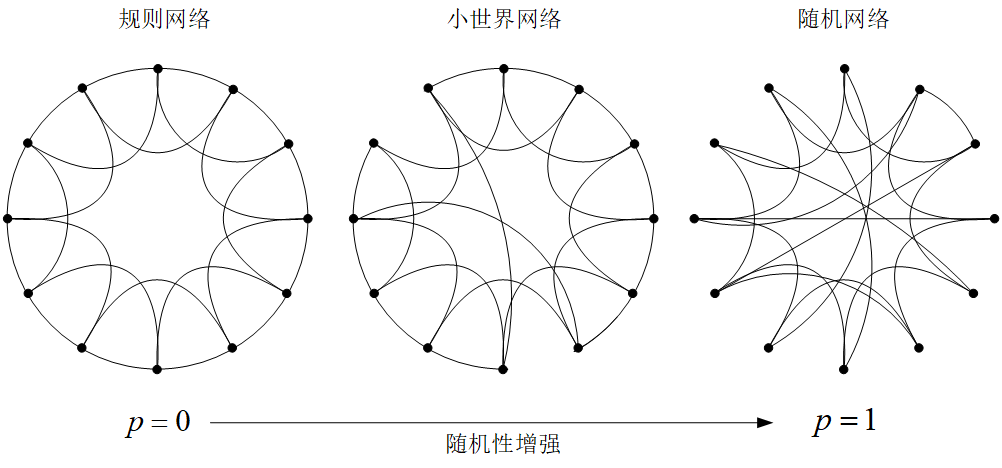
\includegraphics[width=14cm,height=6.5cm]{SW_network.png}
    \caption{小世界网络模型示意图}
    \label{fig:SW}
  \end{figure}

下面进行算例分析,取节点数$N = 1000$,初始网络规则的度$K = 6$,重连概率$p$从0--1依此增加,验证聚类系数$C$和平均距离$L$的变化过程。其验证结果如图\ref{fig:CL}所示。
\begin{figure}[H] % use float package if you want it here
    \centering
    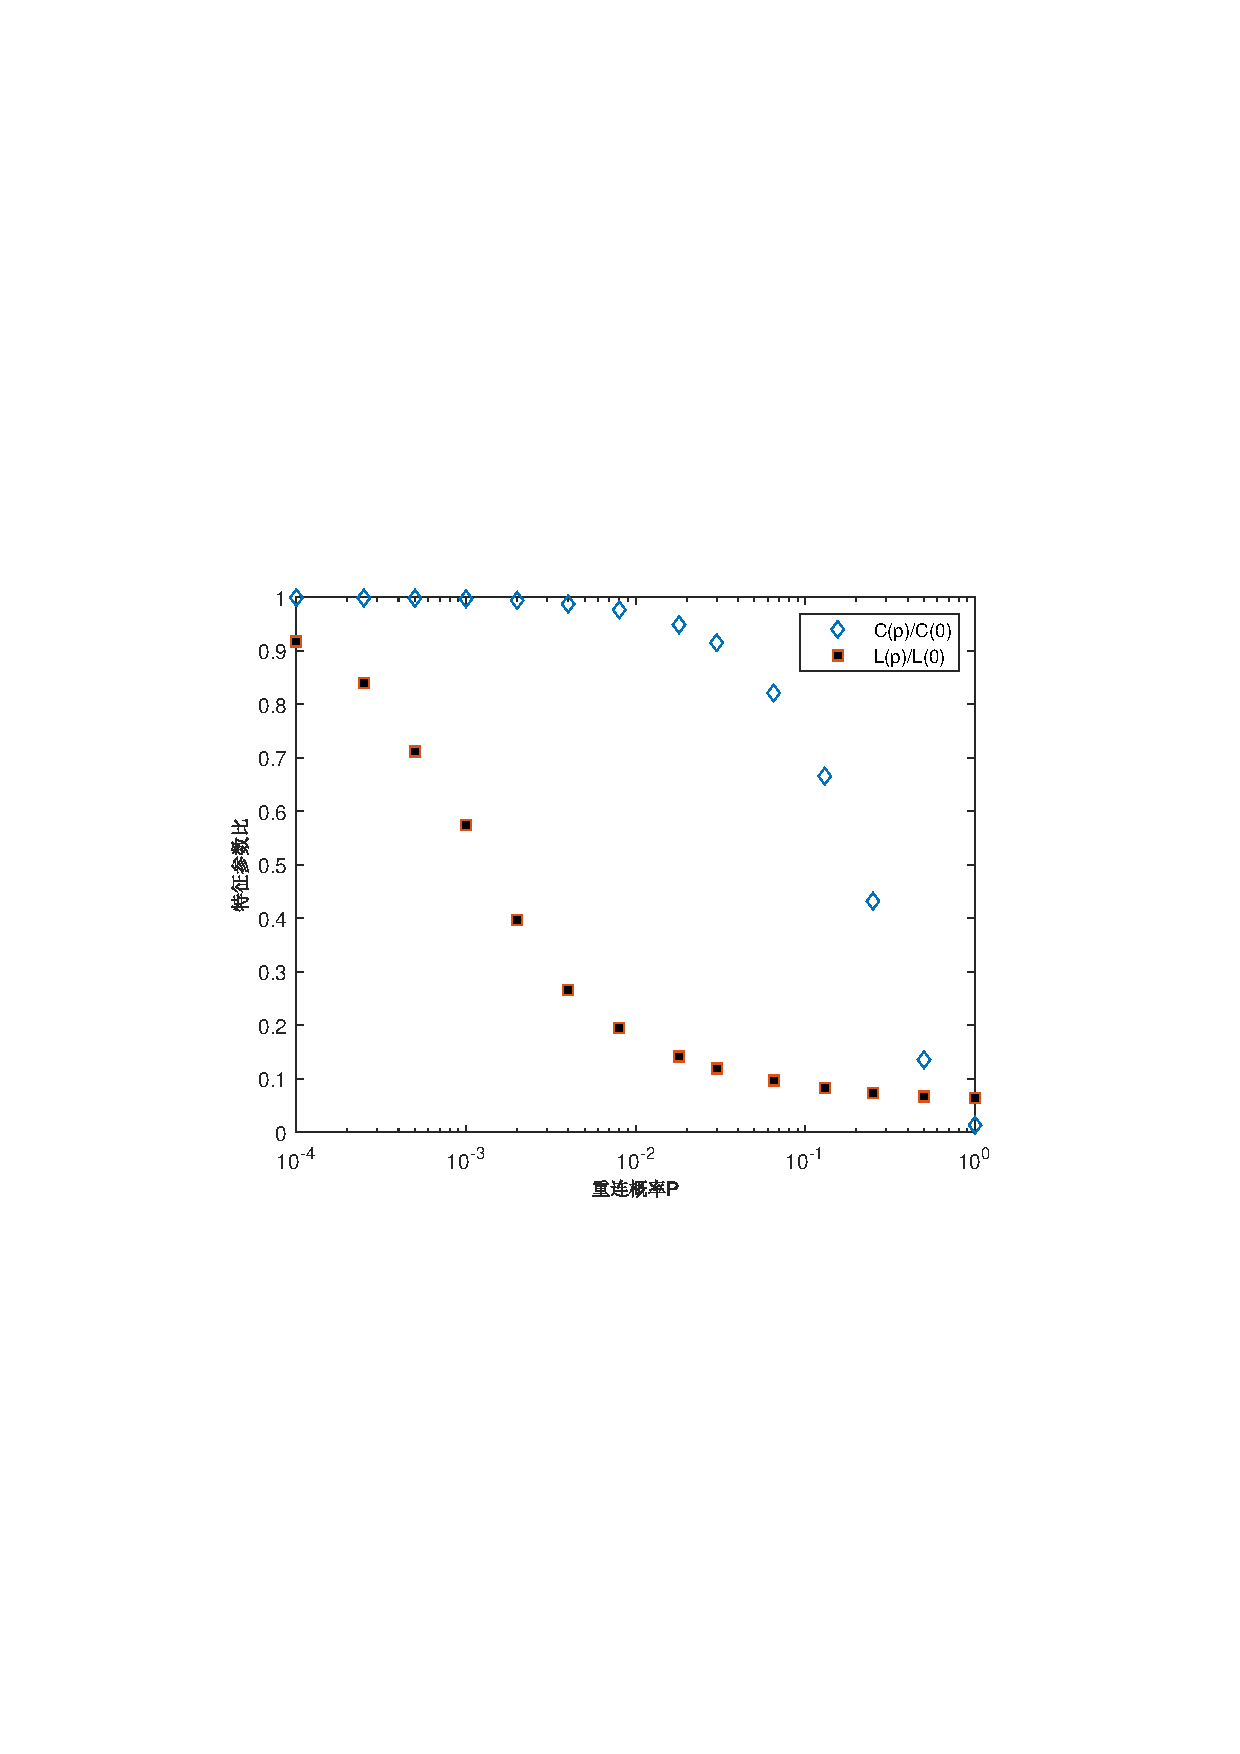
\includegraphics[]{CL.pdf}
    \caption{各重连概率$p$值下聚类系数$C$和平均路径长度$L$的变化趋势}
    \label{fig:CL}
\end{figure}

从图\ref{fig:CL}可以看出,随着重连概率$p$的增加,规则网络经历了从小世界网络到随机网络演变的过程,小世界网络相比于随机网络具有高聚类系数的特征,而相比于规则网络又具有
小平均距离的特征。其表达式如下:
\begin{equation}
\label{equ:chap2:CL}
 C\gg C_{random} \quad \quad\quad L \ll L_{regular}
\end{equation}

小世界网络模型在具体网络的应用方面具有很重要的现实意义。在网络动力学原理中,一般的网络当节点出现故障时,其影响范围很小。而在小世界网络中,由于节点间存在长程连接,节点故障
可能会快速传播到网络其他区域,进而引起网络的连锁故障。小世界网络的特征路径长度和聚类系数与故障传播的深度和广度由密切关系。一般地,特征路径路径长度越小,则故障传播就越深;
聚类系数越大,故障传播就越广\cite{refs41}。

为验证电力系统网络具有小世界特性,下面通过MATLAB工具分别利用$IEEE$30、$IEEE$39和$IEEE$57标准算例模型进行验证,并与相同节点数的规则网络和
随机网络进行对比分析。$IEEE$30、$IEEE$39和$IEEE$57标准算例模型的边数分别为41、46、81。规则网络采用的是最近邻耦合网络,所有的节点只与其最近的$k$个邻居节点相连,因此令规则网络
的边数约等于标准电网模型的边数,$k=2$。并在此规则网络上构建随机网络,重连概率$p$为$1$,取1000次仿真计算结果的平均值为最终值,其仿真结果如表\ref{tab:ieee}、\ref{tab:regular}、\ref{tab:random}所示。
\begin{table}[htb]
    \centering
    \caption{$IEEE$标准算例特征参数计算结果}
    \label{tab:ieee}
      \begin{tabular}{C{3cm}C{3cm}C{3cm}C{3cm}}
        \toprule
        $IEEE$标准算例      & $IEEE$30节点 & $IEEE$39节点 & $IEEE$57节点\\
        \midrule
        聚类系数($C$)       & 0.2348       & 0.0385      & 0.1222 \\
        平均路径长度($L$)   & 3.3057       & 4.7490      & 4.9536 \\
        \bottomrule
      \end{tabular}
  \end{table}

\begin{table}[htb]
    \centering
    \caption{规则网络特征参数计算结果}
    \label{tab:regular}
      \begin{tabular}{C{3cm}C{3cm}C{3cm}C{3cm}}
        \toprule
        规则网络            & 30节点        & 39节点      & 57节点\\
        \midrule
        聚类系数($C$)       & 0             & 0           & 0 \\
        平均路径长度($L$)   & 10.3333       & 13.3333      & 19.3333  \\
        \bottomrule
      \end{tabular}
\end{table}

\begin{table}[htb]
    \centering
    \caption{随机网络特征参数计算结果}
    \label{tab:random}
      \begin{tabular}{C{3cm}C{3cm}C{3cm}C{3cm}}
        \toprule
        随机网络            & 30节点        & 39节点      & 57节点\\
        \midrule
        聚类系数($C$)       & 0.0389       & 0.0275       &  0.0208 \\
        平均路径长度($L$)   & 7.6711        & 8.5568        & 9.1382  \\
        \bottomrule
      \end{tabular}
\end{table}

为了直观显示,规则网络、$IEEE$标准电网和随机网络聚类系数和平均路径长度的对比值如图\ref{fig:Cluster}、\ref{fig:L_mean}所示。
\begin{figure}[H] % use float package if you want it here
    \centering
    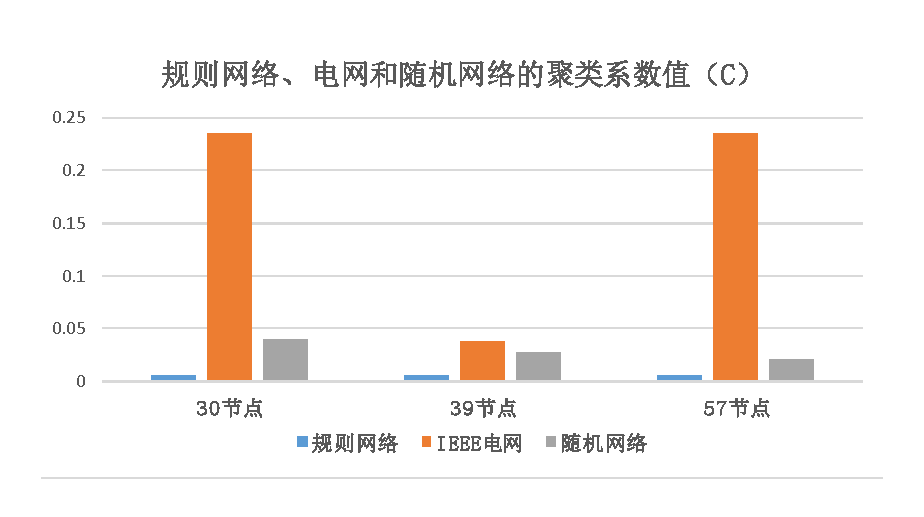
\includegraphics[width=10cm,height=5cm]{Cluster.pdf}
    \caption{规则网络、电网和随机网络的聚类系数结果图}
    \label{fig:Cluster}
\end{figure}

\begin{figure}[H] % use float package if you want it here
    \centering
    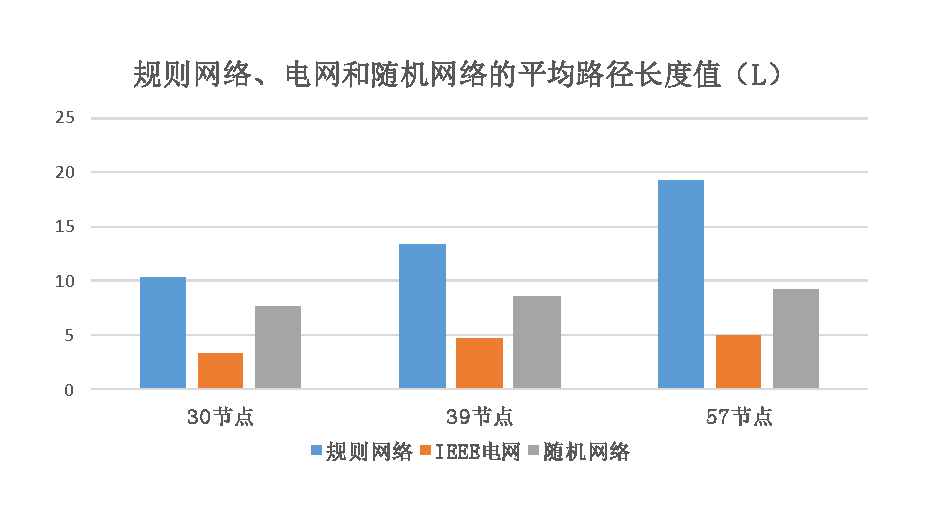
\includegraphics[width=11cm,height=5.5cm]{L_mean.pdf}
    \caption{规则网络、电网和随机网络的平均路径长度结果图}
    \label{fig:L_mean}
\end{figure}

从表\ref{tab:regular}可以看出,在规则网络中,节点30、39、57网络的聚类系数均为0,这是由于每个节点的度数都为2,该规则网络中任意节点的邻居节点都互相不连接,故聚类系数为0。
从图\ref{fig:Cluster}和图\ref{fig:L_mean}验证了式\ref{equ:chap2:CL}的正确性,可以直观看出,实际电网系统的聚类系数远大于随机网络的聚类系数,其平均路径长度远小于规则网络的路径长度,
换言之,电力系统网络相比于随机网络具有高聚集系数的特征,而相比于规则网络又具有小平均距离的特征,因此,验证得到电网模型为小世界网络,具有小世界性。较小的平均距离和较大的聚类系数,在
电网局部发生故障时,其故障具有较大的传播范围和传播速度。这对于研究电网的结构脆弱性具有重要的应用意义。

\subsection{无标度模型}
\label{sec:windModel}
在规则网络中,各节点的度数相同,因此规则网络的度分布集中在一个固定值上。随机网络中,由于其网络的边是以相同概率进行重连的,所以随机网络的度分布大致集中在某个概率区间内。在复杂网络理论中,
大多数现实中的网络的度数呈幂律分布,如式\ref{equ:chap2:milv}所示。因为这些网络的节点没有明显的标度,所以这种网络被称为无标度网络。
\begin{equation}
\label{equ:chap2:milv}
P(k) \propto k^{-r}
\end{equation}

在复杂网络理论中,对无标度网络的鲁棒性进行分析发现,随机攻击对于无标度网络结构的连通性影响很小,而攻击指定的关键环节将会对网络连通性影响很大。在电网中,电网关键节点结构的变化会对网络的连通性
造成极大的影响,进而影响电网的运行状态导致负荷损失\cite{refsBA}。因此,无标度网络中的关键环节可视为电网模型的脆弱环节。下面将验证电网模型的无标度性。

本文选取$IEEE13659pegase$节点标准算例进行实验,通过$MATLAB$计算电网模型中各节点的度,进而得到电网的度分布结构,实验结果如图
\ref{fig:dufenbu}所示。
\begin{figure}[H] % use float package if you want it here
  \centering
  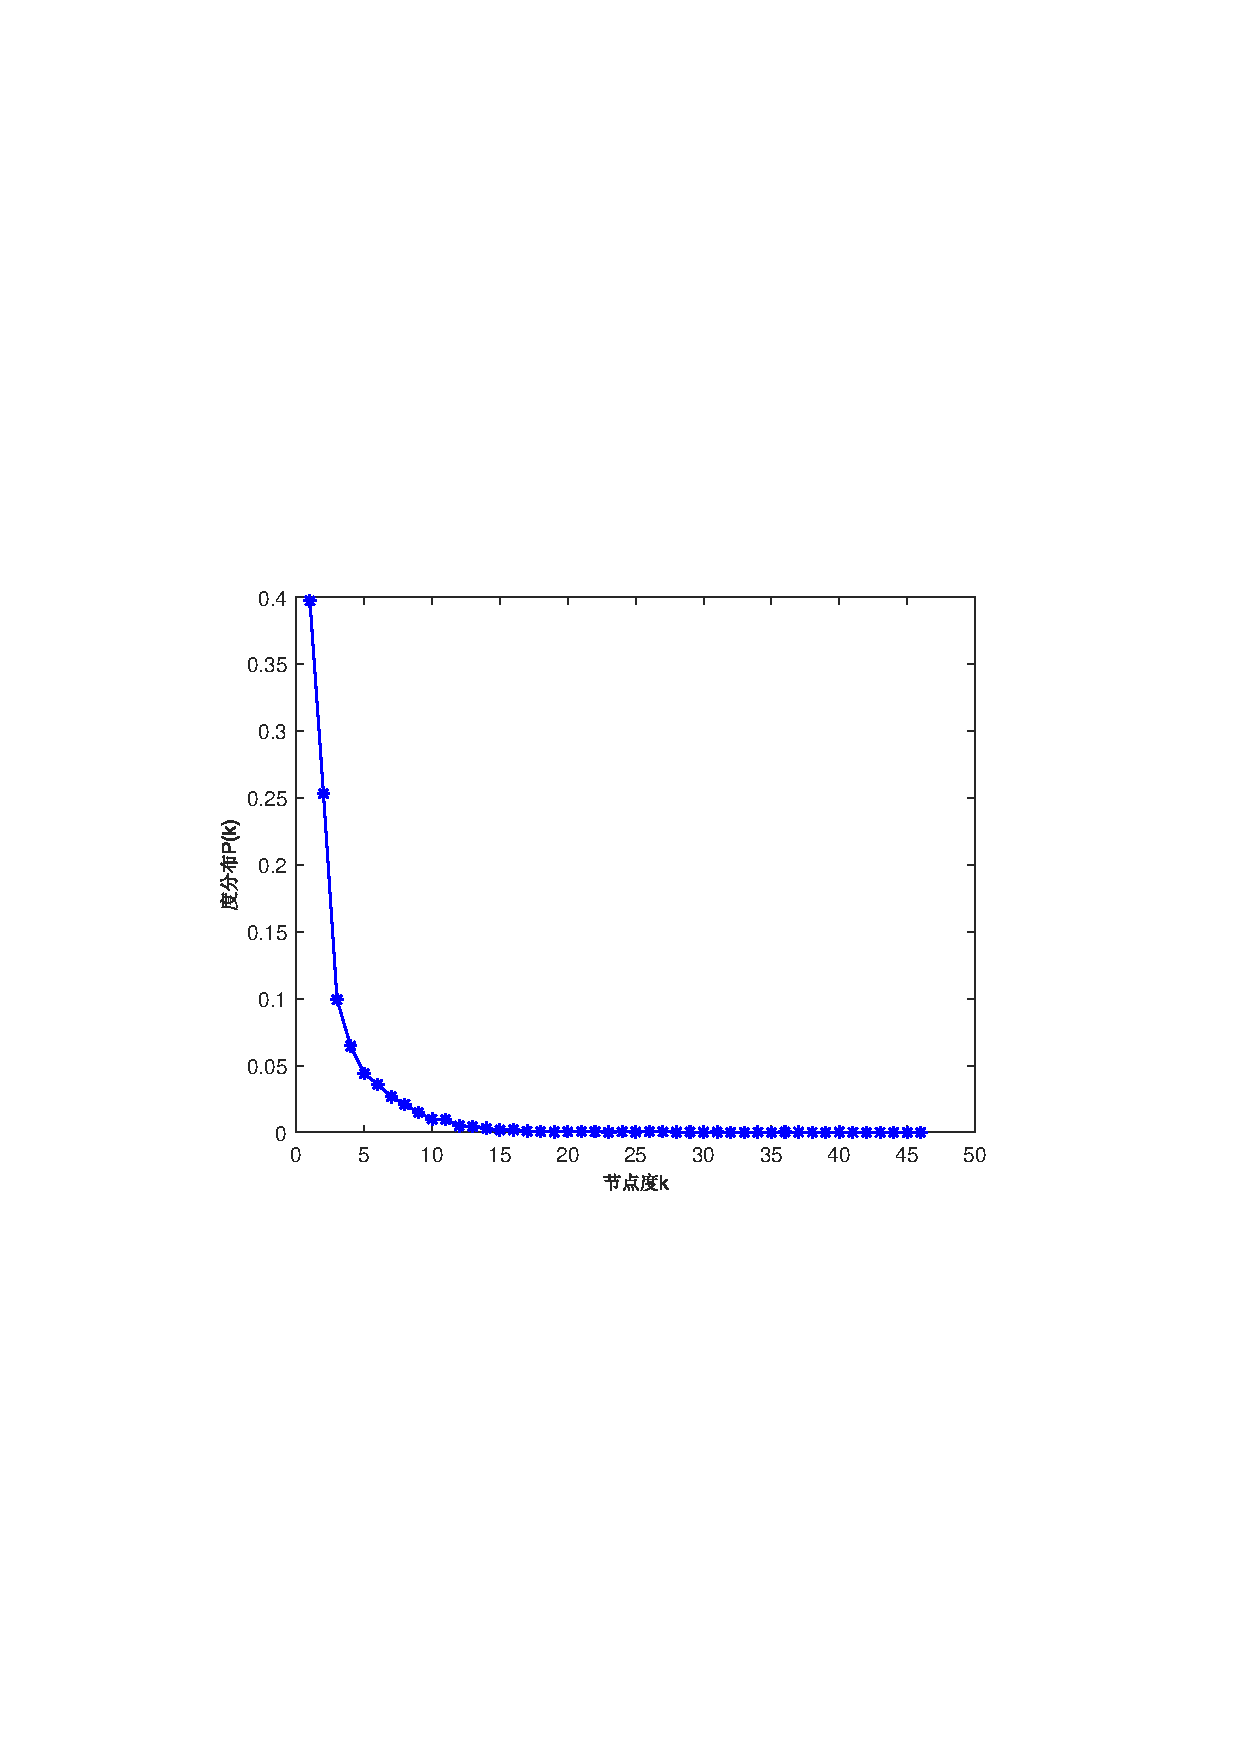
\includegraphics[width=11.61cm,height=9.15cm]{dufenbu.pdf}
  \caption{$IEEE13659pegase$标准算例节点度分布图}
  \label{fig:dufenbu}
\end{figure}

从图\ref{fig:dufenbu}可以看出,将近$40\%$节点度为1,节点度为2的占到了$25\%$以上,节点度为3的约占$10\%$,剩下的约占$25\%$,下面对$IEEE13659pegase$标准算例节点度分布进行幂函数拟合。
其拟合结果如图所示。
\begin{figure}[H] % use float package if you want it here
  \centering
  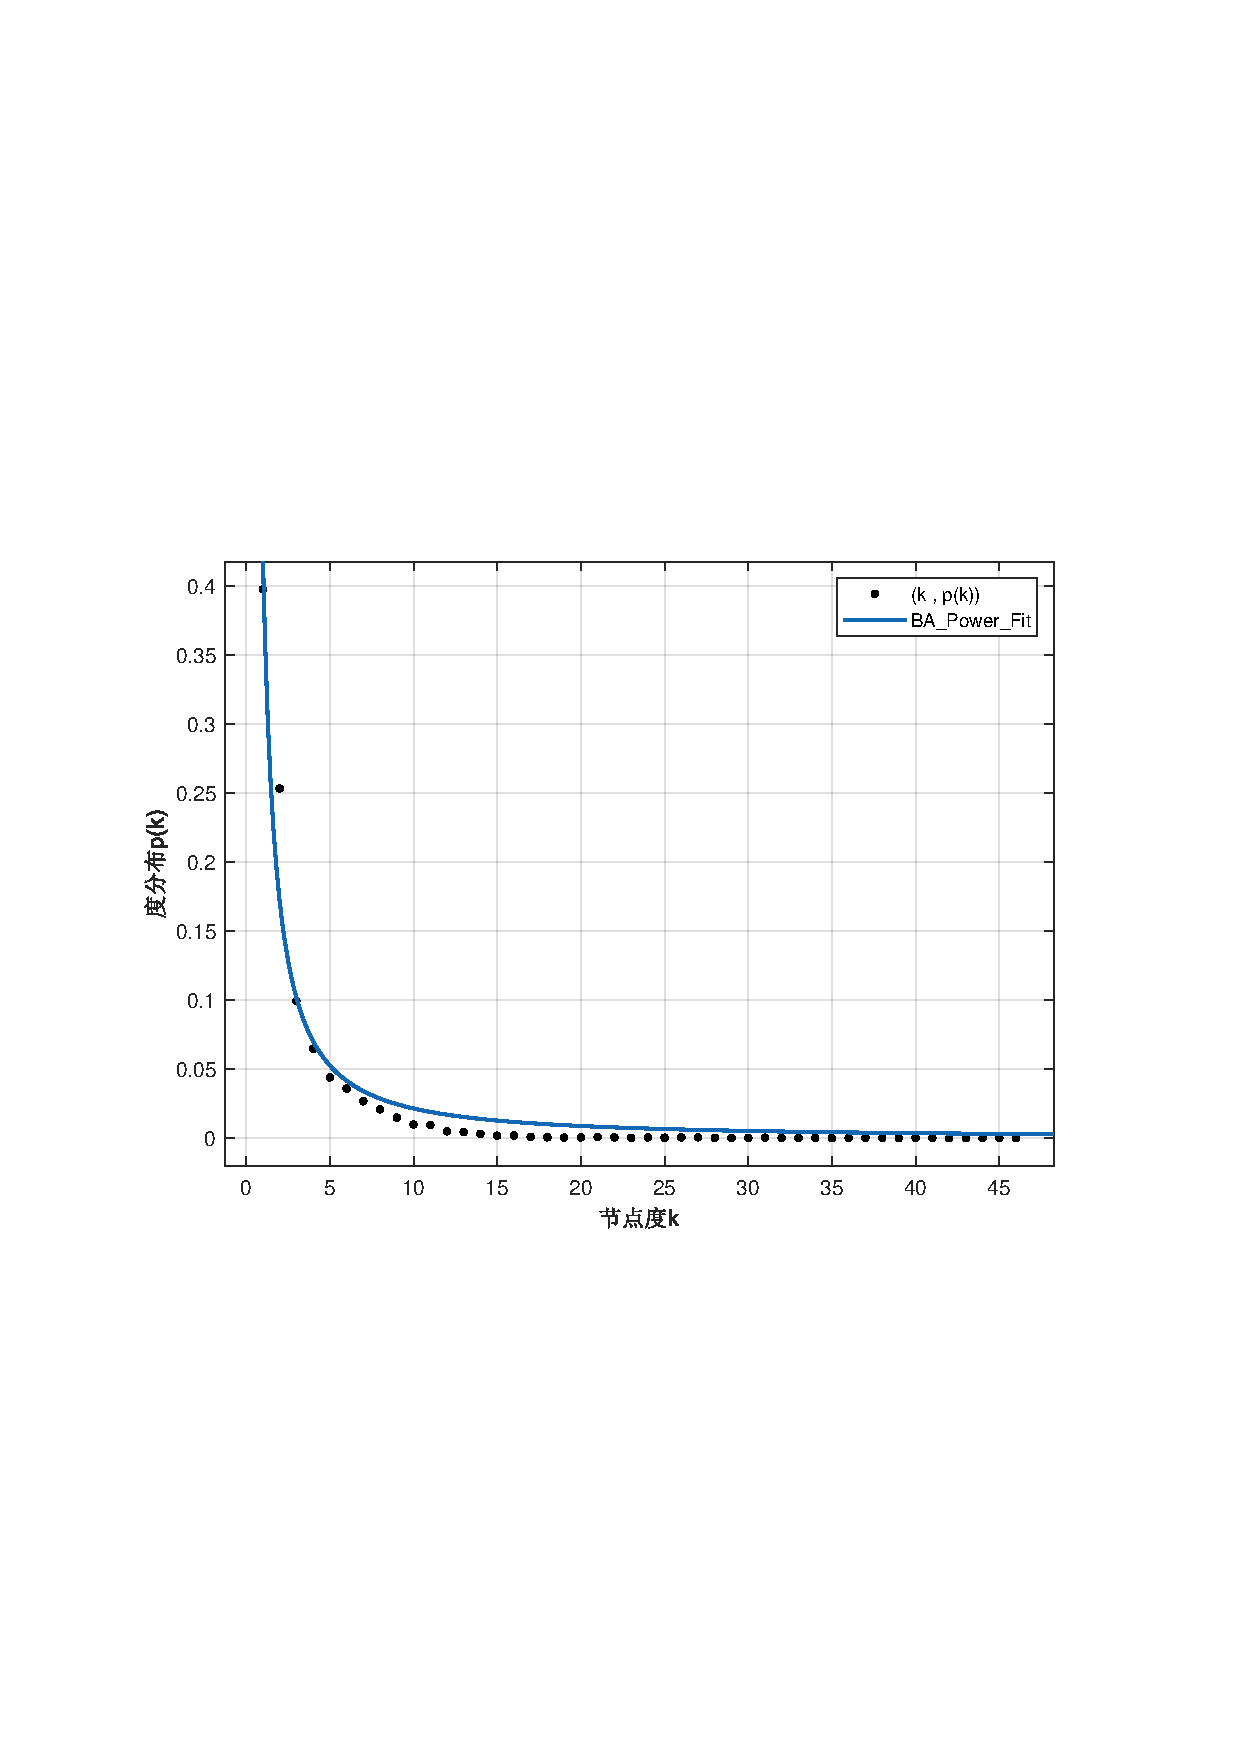
\includegraphics[width=11.61cm,height=8.48cm]{power_fit.pdf}
  \caption{$IEEE13659pegase$标准算例节点度分布拟合图}
  \label{fig:fower_fit}
\end{figure}

利用$IEEE13659pegase$标准算例,得到其度分布示意图,其趋势变化服从幂律分布,对数据进行数据拟合得到$p(k)=a k^{b}(a=0.4206, b=-1.292)$ 置信度为$95\%$。

无标度特性反映出电网具有严重的异质性,其各节点之间的连接状况(度数)具有严重的不均匀分布性:网络中少数称之为Hub点的节点拥有极其多的连接,而大多数节点只有很少量的连接。
少数Hub点对无标度网络的运行起着主导的作用。从广义上说,无标度网络的无标度性是描述大量复杂系统整体上严重不均匀分布的一种内在性质。这也表明了电网作为无标度网络的一种,当其面临蓄意的节点
攻击时较为脆弱,面临随机攻击时鲁棒的特点。
%通过验证电网的无标度特性,对本文提出脆弱性指标和研究电网结构脆弱性具有重要意义。

\section{复杂网络脆弱性概念与电网脆弱性的关键问题}
\label{sec:load}
通过上节\ref{sec:complexGrid}对标准算例系统的性质验证可知,电网具有小世界性和无标度性,属于典型的复杂网络。本节就复杂网络的脆弱性概念进行研究分析,明确电网脆弱性研究的关键问题。

\subsection{复杂网络脆弱性概念分析}
\label{sec:loadEffect}
复杂网络的脆弱性是指:对于一个复杂网络$S$,存在一个子系统$S_i$,对环境有强烈的敏感性,当$S_i$受到内、外因素(包括信息、物质流等因素)的扰动或攻击产生崩溃时,会使其他部分或子系统也产生崩溃,
进而导致整个复杂网络崩溃\cite{refs31}。复杂网络所具有的这一特性称之为复杂网络的脆弱性。

从以上复杂网络的定义可以看出,复杂网络大致有元素、关系、环境组成。其中元素是复杂网络中的各子系统,而关系包括元素与网络的关系、元素之间的关系、元素与环境的关系等;环境是指一切与系统关联的
事物的集合,比如外界扰动。复杂网络脆弱性研究的是在系统的某一元素受外界干扰引起崩溃后,其他子系统和整个网络的变化,研究重点是在不确定性环境中,各元素之间,元素与整体之间、元素与环境之间
以及整体与环境之间的关系。

\subsection{电网脆弱性研究的关键问题}

复杂网络的脆弱性主要在于子系统的存在性,即存在能够引起系统崩溃的子系统,如何识别这样的子系统是复杂网络脆弱性研究的重要方向。本文依照复杂网络脆弱性的研究思路,研究元素与整体之间
的关系,即电网节点与电网整体性能之间的关系,分析电网各节点对于电网整体的重要程度,进而量化分析系统中各节点的脆弱性。因此,建立电网脆弱性综合评估模型,识别电力系统的脆弱环节成为
本文电网脆弱性研究的关键问题。

% \subsection{电力系统整体性能指标}
% \label{sec:loadModel}
% 在研究系统节点对电网整体的影响程度以及重要性时,需要选取电网整体性能指标来进行量化。因此,本文从网络连通性和传输效率的角度考虑,基于复杂网络选取网络结构熵和网络平均效率作为电网的整体性能指标。

% $(1)$网络结构熵

% 熵(Entropy)是系统的一种无序的度量。如果网络是随机连接的,各节点的度分布大致相当,则认为网络是无序的;反之,如果网络是无标度的,网络中有少量的具有高连通度的中枢节点和大量低连通度的节点,
% 在这方面可以看出,节点的重要程度存在差异,可认为这种网络是有序的。网络结构熵定义可以简洁地度量电力系统的有序程度。

% \begin{definition}
%   假设网络中的节点$v_i$的度为$k_i$,则其重要度可以定义为\cite{refsNetShang}
% \end{definition}
% \begin{equation}
%   I_{i}=\frac{k_{i}}{\sum_{j=1}^{N} k_{j}}
% \end{equation}

% 对于$k_i = 0$的节点不做考虑,可以定义网络结构熵为
% \begin{equation}
% \label{equ:chap2:shang1}
%   E_{entropy}=-\sum_{i=1}^{N} I_{i} \cdot \ln I_{i}
% \end{equation}

% 从式\ref{equ:chap2:shang1}可得,当网络完全均匀时,如图\ref{fig:netEntropy1}所示,即$I_{i}=1 / N$时,$E_{\max }=\ln N$。当网络中所有节点都与某一个中心节点相连,假设所有节点都与节点$i$
% 相连,如图\ref{fig:netEntropy2}所示,即$k_i = N-1$,$k_j = 1(j \neq i)$时,网络最不均匀,此时网络结构熵最小,$E_{\min }=\ln [4(N-1)] / 2$,根据网络结构熵的最值可进行标准化。
% \begin{figure}[H] % use float package if you want it here
%   \begin{minipage}[t]{0.5\linewidth}
%   \centering
%   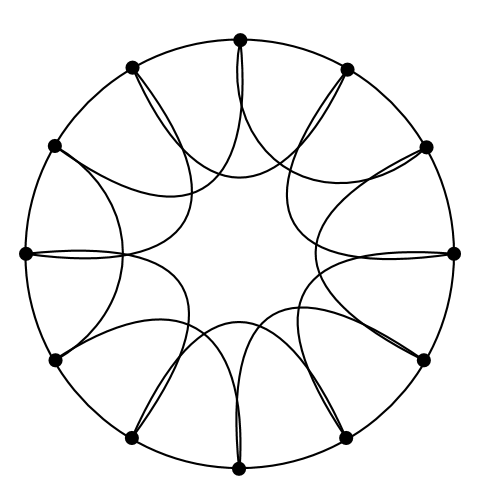
\includegraphics[width=5cm,height=5cm]{netEntropy1.png}
%   \caption{规则网络结构图}
%   \label{fig:netEntropy1}
%   \end{minipage}
%   \begin{minipage}[t]{0.5\linewidth}
%   \centering
%   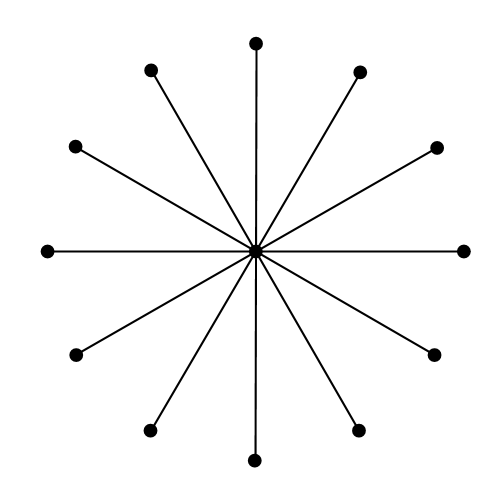
\includegraphics[width=5cm,height=5cm]{netEntropy2.png}
%   \caption{不规则网络结构图}
%   \label{fig:netEntropy2}
%   \end{minipage}
% \end{figure}

% 根据上述结构熵的定义可知,当电力系统网络具有无标度性时,其值会相对较小,此时网络的连通性较好。当网络受损或节点遭受破坏时,电力系统会发生裂解,其熵值会变大。因此,网络结构熵可以衡量
% 网络连通性以及为验证网络核心节点提供度量,识别电力系统中的脆弱环节,对于保护整个电力系统网络具有重要的指导价值。

% $(2)$网络平均效率

% 在衡量网络信息传输效率方面,平均路径长度可作为一个重要评价参数,对于一个$N$个节点的复杂网络,其表达式为
% \begin{equation}
%   L=\frac{1}{C_{N}^{2}} \sum_{1 \leq i<j \leq N} d_{i j}
% \end{equation}

% 由于网络有些节点对处于非连通状态,因此路径长度会出现无穷大的情况,影响后续的研究分析。为了避免这种情况的发生,在研究网络结构脆弱性方面,采用网络平均效率$E_{mean}$代替平均路径长度$L$。
% 描述的是:节点间传输单位能量,沿最短路径传播时的效率,该指标用于描述整个网络能量传递的效率。表达式如下
% \begin{equation}
% \label{equ:cahp2:netEfficiency}
%   E_{mean}=\frac{1}{N(N-1)} \sum_{i \neq j} \frac{1}{d_{i j}}
% \end{equation}

% 式\ref{equ:cahp2:netEfficiency}中,$N$为网络节点的个数;$N(N-1)$为所有的节点对个数;$d_{ij}$为节点$i$、$j$间的最短路径距离,若节点$i$、$j$不可达,则 $d_{i j}=\infty$。

\section{本章小结}
\label{sec:sum2}
本章基于复杂网络理论,分析了复杂网络的概念和特征参数,以$IEEE$30、39、57标准电网模型为例,通过MATLAB计算电网模型参数并进行数据拟合得到,电力系统具有高聚类系数,短平均距离的特点,
并且其节点度数呈幂律分布,验证了电力系统的小世界性和无标度性,这对于电力系统脆弱性研究具有重要意义,通过对复杂网络脆弱性概念的研究,明确了本文对于电网脆弱性研究的关键问题。




